%
% domain.tex -- domain graph for problme 30000018
%
% (c) 2019 Prof Dr Andreas Müller, Hochschule Rapperswil
%
\documentclass[tikz,12pt]{standalone}
\usepackage{amsmath}
\usepackage{times}
\usepackage{txfonts}
\usepackage{pgfplots}
\usepackage{csvsimple}
\usetikzlibrary{arrows,intersections,math}
\begin{document}
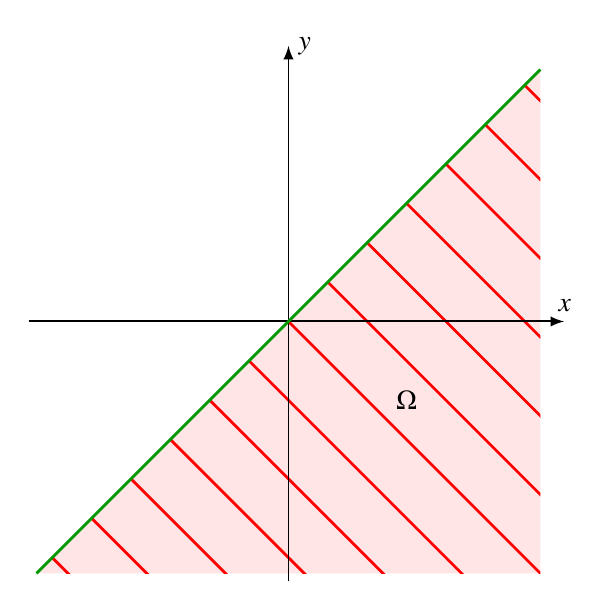
\begin{tikzpicture}[>=latex]

\definecolor{darkgreen}{rgb}{0,0.6,0}

\fill[color=red!10] (-3.2,-3.2)--(3.2,-3.2)--(3.2,3.2)--cycle;

\begin{scope}
\clip (-3.2,-3.2) rectangle (3.2,3.2);
\foreach \s in {-3,-2.5,...,3}{
	\draw[line width=1pt,color=red] ({\s},{\s})--({\s+7},{\s-7});
}
\end{scope}

\node at (1.5,-1) {$\Omega$};

\draw[->,line width=0.7pt] (-3.3,0)--(3.5,0) coordinate[label={$x$}];
\draw[->,line width=0.7pt] (0,-3.3)--(0,3.5,0) coordinate[label={right:$y$}];

\draw[line width=1pt,color=darkgreen] (-3.2,-3.2)--(3.2,3.2);

\end{tikzpicture}
\end{document}

